\documentclass{article} % For LaTeX2e
\usepackage{nips13submit_e,times}
\usepackage{hyperref}
\usepackage{url}
\usepackage{graphicx}
\usepackage{amsmath}
\usepackage{float}
\usepackage{subfigure}
\usepackage{color}
%\documentstyle[nips13submit_09,times,art10]{article} % For LaTeX 2.09


\title{Traffic Flow Maximization using Evolutionary Algorithm}


\author{
Cui Jiaxing \\
ECE Department\\
Carnegie Mellon University\\
Mountain View, CA \\
\texttt{jiaxingc@andrew.cmu.edu} \\
\And
Quentin de Metz \\
ECE Department \\
Carnegie Mellon University\\
Mountain View, CA \\
\texttt{qdemetz@andrew.cmu.edu} \\
\AND
  \\
\And
  \\
}


\newcommand{\fix}{\marginpar{FIX}}
\newcommand{\new}{\marginpar{NEW}}

\begin{document}

\maketitle

\begin{abstract}
Traffic Flow maximization is one of the crucial problems in designing a city. It directly affects the daily life of the people living in that city. It is a complex problem, one that in most cases cannot be deterministically solved. We propose using evolutionary algorithms to solve that problem. We compare existing work and traffic flow with solutions yielded by our evolutionary approach, and our results show that it is beneficial to adopt this strategy when designing traffic light timings.
\end{abstract}
\textbf{Keywords:} \hspace{0.2em} Evolutionary Algorithm, Traffic Light Optimization
\section{Scope of the Problem}

Traffic infrastructure comes in various forms, and optimizing traffic flow in road networks is a task that depends highly on the infrastructure. We commonly consider infrastructure as being in one of two categories:  ``smart'' infrastructure and ``legacy'' infrastructure. The first makes use of detectors placed in the infrastructure to determine the state of traffic, whereas the second does not.

It is reasonable to assume that achieved solutions will perform better as a whole when making use of smart infrastructure. For example, a traffic light that can detect that there is no traffic from East to West, and that vehicles are waiting to go from North to South, can react accordingly and change its state to shorten the wait of these vehicles.

There have been projects in the past where traffic flow was optimized by combining real-time knowledge of traffic and communication between lights. The best-known of these projects is one spearheaded by Carnegie Mellon University in the East Liberty part of Pittsburgh, with excellent results.

However, this previous study's approach relies heavily on smart traffic lights and detectors, which, although quite practical, are still far and few between throughout the world. In countries such as China or India, where the number of vehicles is growing most rapidly, most roads are equipped with legacy traffic equipment.

An effective approach to solving this problem should be applicable to the maximum amount of scenarios, which is why this paper discusses only optimizing traffic light timings in a legacy environment.
However, operating in a legacy environment does not mean that we must forgo all knowledge of the traffic flow. It is reasonable to assume that traffic flow can be measured at specific intersections. The collection of this data can unearth trends in the traffic flow (ie: rush hour traffic). Once this data is collected, any period of time can be split into different sections, where each of these sections has a different, but constant, traffic flow.


In our analysis, we place ourselves in an environment where the traffic flow is a fixed parameter. The above analysis shows that this scenario is relevant.

\section{Existing Domain Research}
Researchers have come up with several different ways to optimize traffic lights in the past. Many studies have focused on adding sophisticated detectors at intersections, or on adding features to the traffic lights to leverage existing traffic theory results and artificial intelligence once the lights are capable of transmitting the state of the intersection to their neighbors. This approach is the one pursued by Ken Walters of Carnegie Mellon University and has produced good results ([1]).

Jansson used evolutionary algorithms to optimize traffic, but only in the context of one traffic light. He produced a microcontroller implementation for his simulator and his results state that his evolutionary approach yielded better results than a deterministic approach as soon as the problem reached a certain size ([3]).

Sanchez Medina has used evolutionary algorithms to evolve traffic light timings on several major streets throughout Spain. They implemented a Standard Genetic Algorithm based on truncation and elitism. Although their paper deals talks mostly about designing and programming a custom simulator, their conclusions state that they produced good (but not great) results during their experiments ([4]).


\section{Simulators}
A common and key ingredient in developing evolutionary algorithms is the choice of a simulator. We investigated several traffic simulators (see below) and chose the one that suits our project the best.
\subsection{Simple Java Simulator}
This Java simulator showed in Figure \ref{fig:simulator_java} can automatically generate and plot. Another feature is the ability to to drag any car from one position to another. The simulator will automatically adjust the position of the car and continue. Furthermore, it is possible to adjust in real-time the timings of traffic lights. For simple road networks and light traffic flow, it is a great choice. However, in this kind of traffic network, there isn't much to optimize, which is why we didn't choose it as our final simulator. 
\subsection{MatSim}
Matsim showed in Figure \ref{fig:simulator_matsim} is a powerful simulator which you can see from its simulated traffic networks. It is open source, which means that developers can modify it as they wish and adapt it closely to their needs. Also it provides and interactive visualizer which enables users to modify the traffic networks conveniently. At the same time, it provides detailed analysis which can be used by our project.
\subsection{SUMO}
After comparing carefully among several different simulators, we finally chose SUMO which was developed by employees of the Institute of Transportation Systems at the German Aerospace Center. Figure \ref{fig:sumo} shows how it looks like. It can handle complex situations and have a good perform even when the number of cars is very large. Also it can deal with collisions, acceleration and deceleration.

\section{Simulated Traffic Networks}
In order to test our algorithm, we modeled the traffic network around the Caltrain station located in Mountain View, California. This choice was informed by the fact that it is a well-known intersection among our peers and we have heard complaints about its long wait times. We investigated the traffic situation around the Caltrain station: during rush hour, we recorded the traffic flow as well as the traffic light timings. Figure \ref{fig:sumo} shows the traffic network around Caltrain Station.

%differnt kinds of simulator
\begin{figure}[h]
 \centering
  \subfigure[Java Simulator]{ \label{fig:simulator_java}
   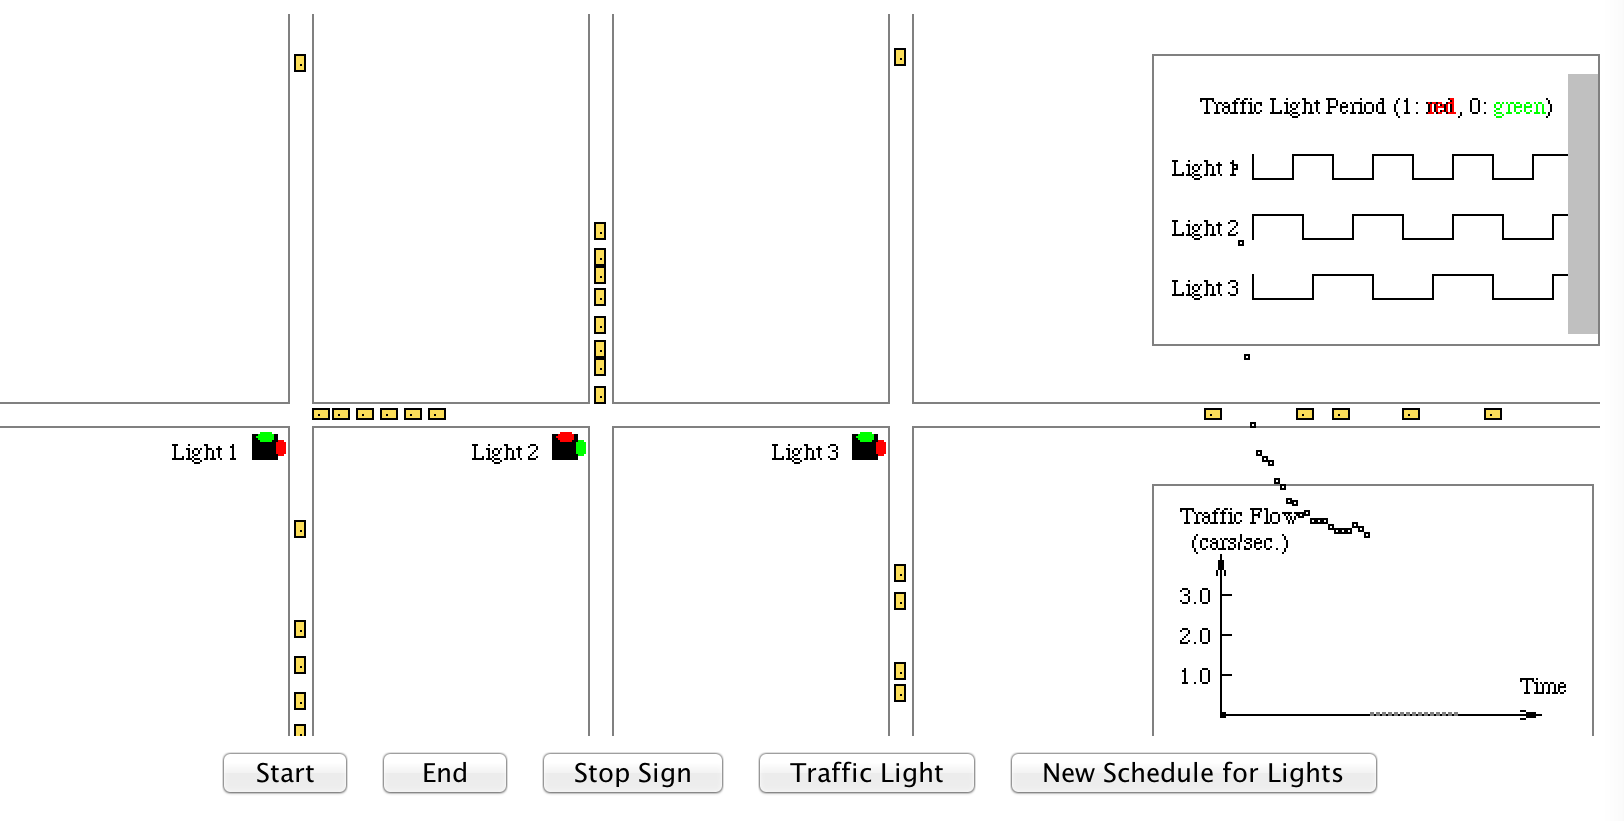
\includegraphics[width=0.45\textwidth]{images/simulator/SimpleJavaSimulator.png}}
  \subfigure[Matsim]{ \label{fig:simulator_matsim} %% label for second subfigure 
  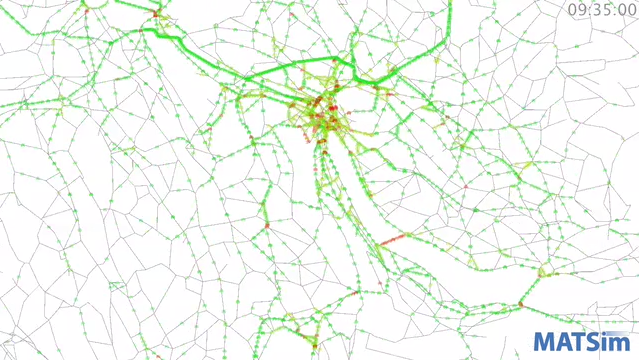
\includegraphics[width=0.45\textwidth]{images/simulator/matsim_zurich.png}}
  \subfigure[SUMO]{ \label{fig:sumo} %% label for second subfigure 
  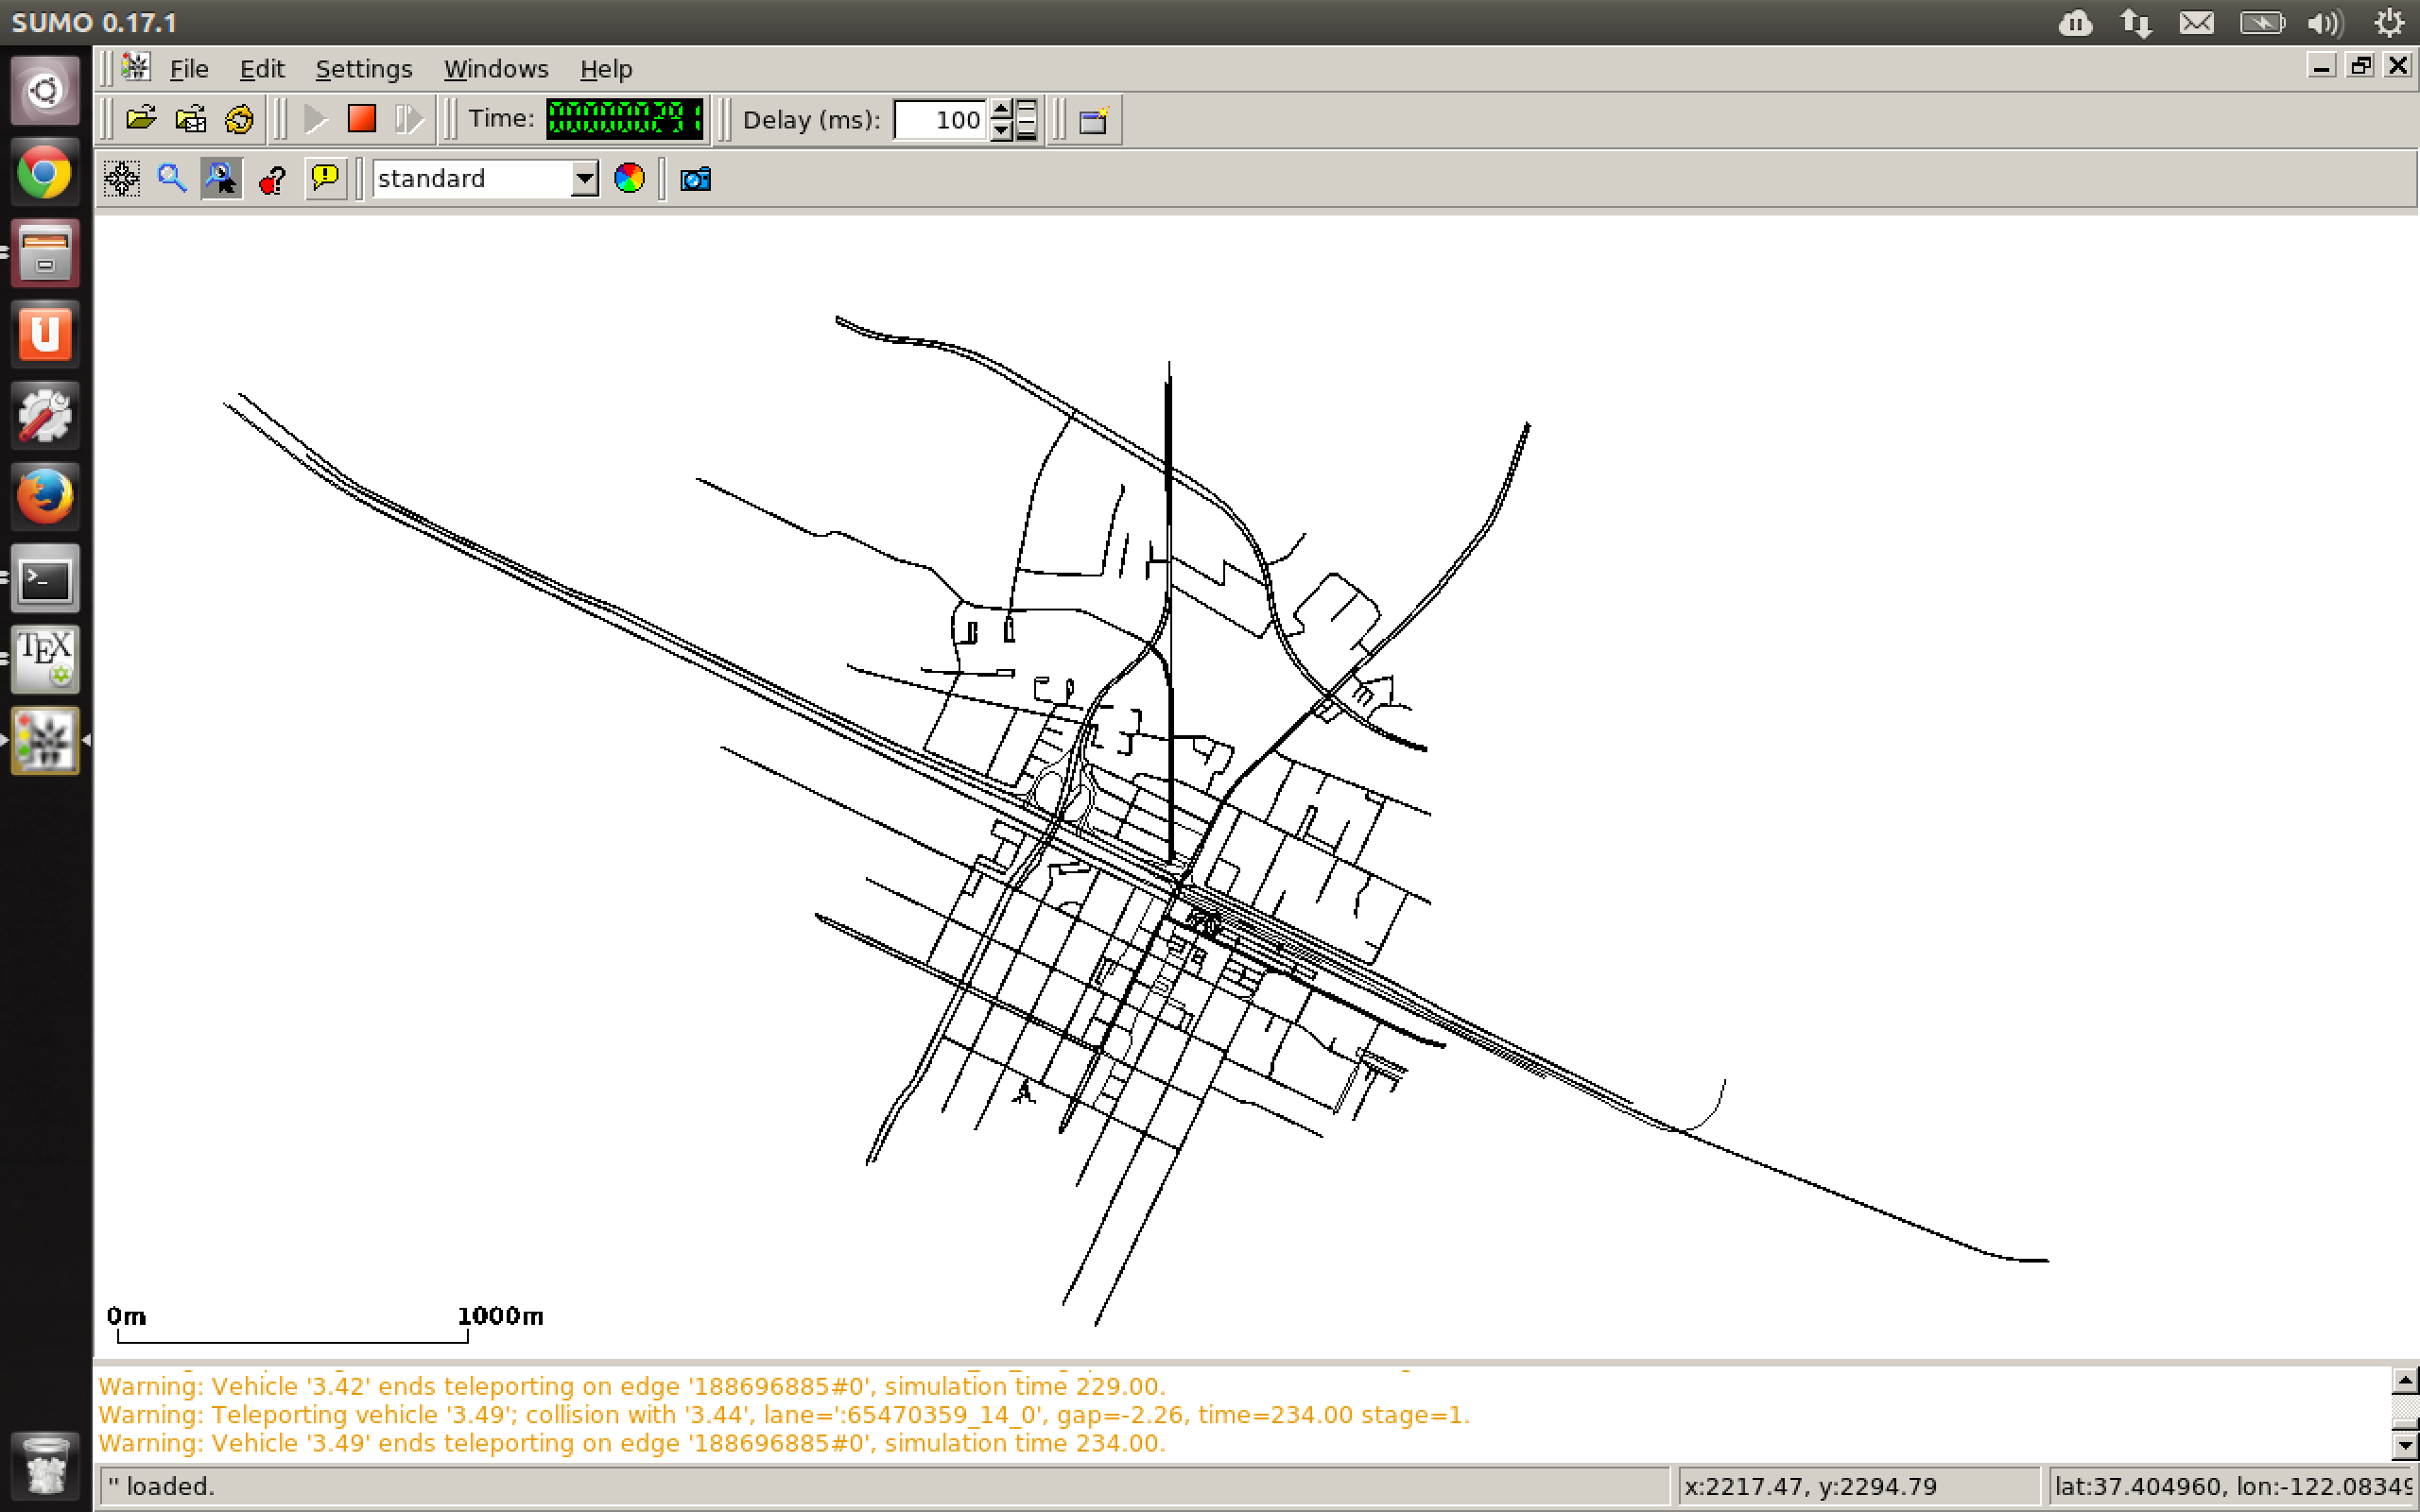
\includegraphics[width=0.75\textwidth]{images/simulator/caltrain.png}}
  \caption{Simulators}
   \label{fig:simulator} %% label for entire figure 
\end{figure}


\section{Fitness Function}
In order to best simulate the real world traffic light, we tried several ways to establish the mapping between real world traffic measurement with the fitness function in our evolutionary algorithm. The following are the fitness function we tried in our algorithm.
\subsection{Average Speed}
The first fitness function we designed was the average speed of the vehicles in the network. This is an intuitive metrics, in that if the average speed of a traffic network is larger than that of another, then we can expect its traffic flow to be equally larger. We used this fitness function when testing our algorithms in the grid traffic network.%, as shown in figure~\ref{fig:gridoptimum}.

However, this fitness function did not fit well with the simulator we were using. Indeed, the SUMO simulator had no easy means of recovering the average speed of a vehicle at a given time. In the above experiment we had resorted to placing detectors at specific places along the network; these detectors could measure the velocity of vehicles passing next to them (think of them as speed radars). Whereas this approach worked well in a simple traffic network, placing a number of detectors along multiple roads in a real-world, intricate network was a tedious task. Furthermore, our fitness function was not detector-location agnostic, which means that the placement of the detectors directly impacted the fitness values that we measured, and in turn could greatly impact the results of our algorithms. We decided to move on to a simpler fitness function.

%\begin{figure}[h]
%\centering
%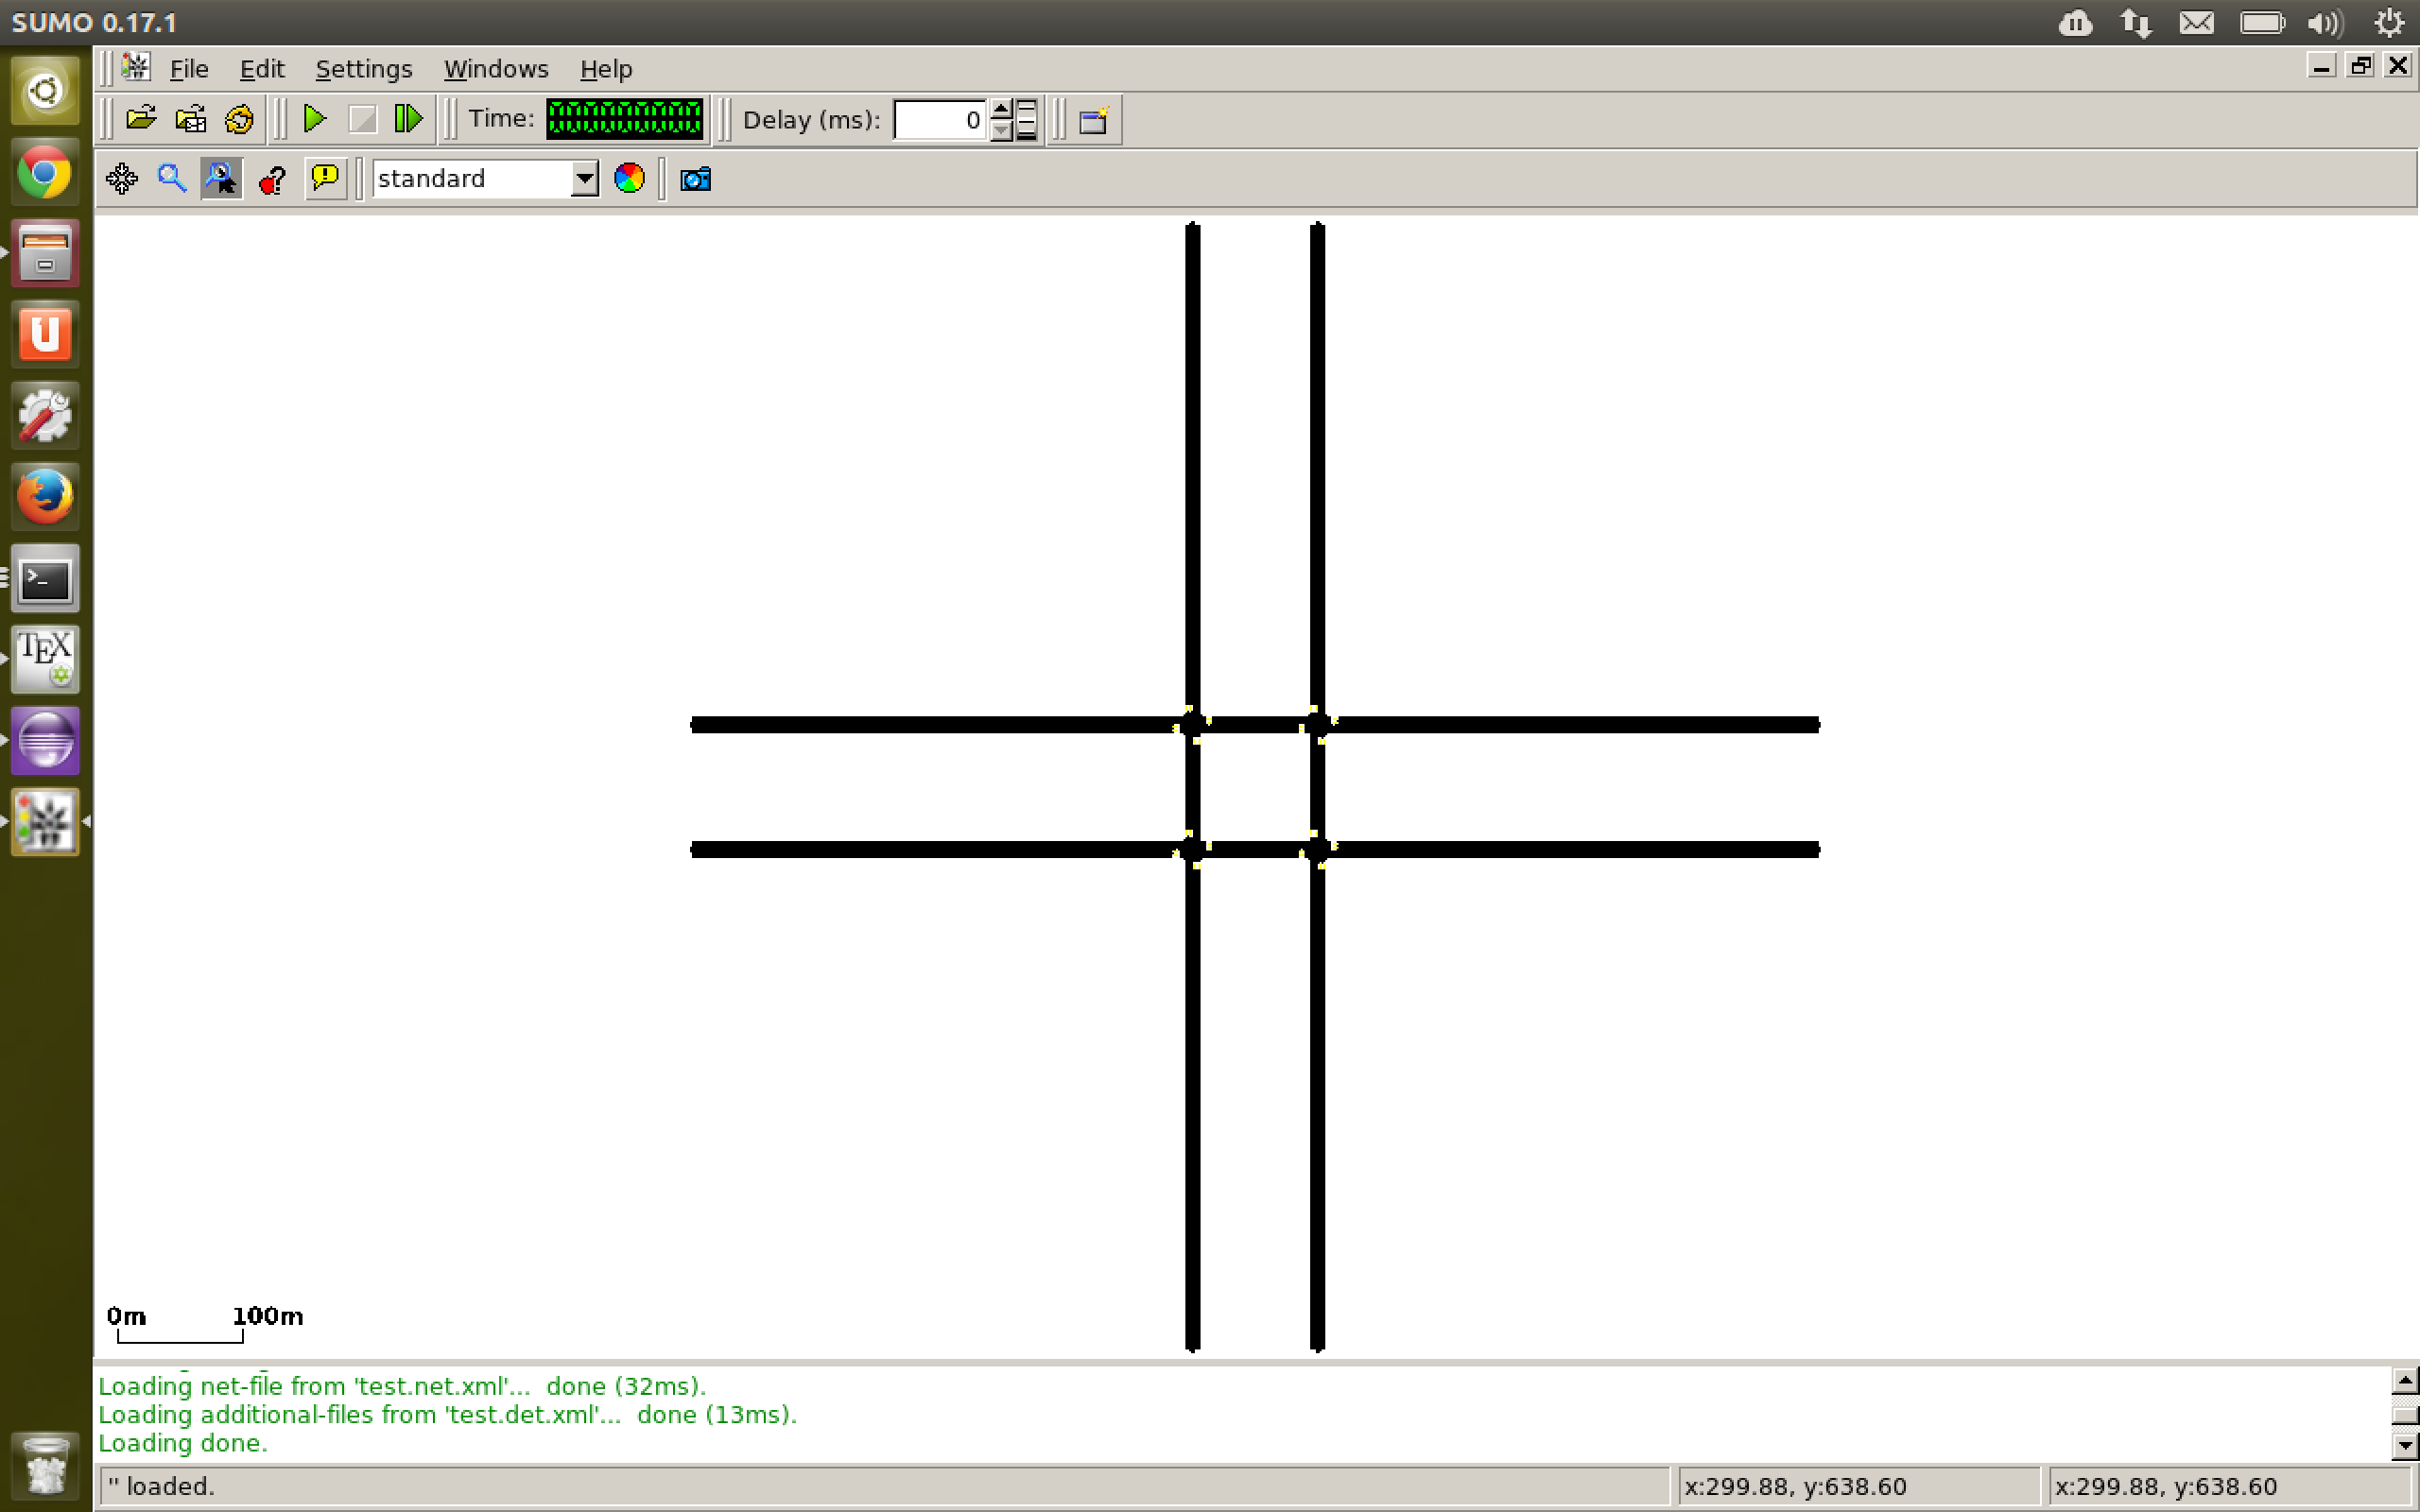
\includegraphics[width=0.5\textwidth]{images/simulator/gridoptimum.png}
%\caption{Basic Simulation}
%\label{fig:gridoptimum}
%\end{figure}

\subsection{Throughput}
When modelizing the traffic flow in the simulator, we created many different routes that the vehicles would use. When the simulator placed a new vehicle in the network, it chose an a path for the vehicle from within a list of predermined paths that we had decided upon. It made sense to evaluate how many vehicles were making it to their destination in the fixed, allocated time that our simulation was running in, and we chose this as a metric for our fitness function. Intuitively, it is related to the throughput of the traffic network.

This fitness function was much simpler to implement on larger, more complex networks. However, we noticed one significant drawback: not all paths had equal length, nor an equal number of traffic lights on them. This meant that the algorithm tended to optimize the network for paths that were shorter (an easier target because there were less traffic lights to optimize). This bias affected the early results of our algorithms, but we nonetheless managed to achieve significant results.

\section{Algorithms}

\subsection{Simple GA}

\subsubsection{Overview}
The first algorithm which we implemented was the Simple Genetic Algorithm. This textbook algorithm is made of several components, among which the following:
\begin{itemize}
 \item Parent Selection
 \item Recombination
 \item Mutation
 \item Survivor Selection
\end{itemize}
Each of these components can be implemented in different ways and will give the algorithm a unique behavior. Furthermore, these components make use of constants that can be tweaked (mutation rate, parent population size), just as the algorithm's parameters (population size, number of rounds). Tuning these values will also change the behavior of the alorithm.

Our implementation contains the following components:
\begin{itemize}
 \item Parent Selection: Rank-based selection, Stochastic Universal Sampling
 \item Recombination: Single Point Crossover
 \item Mutation: Simple Mutation: replacing one traffic light by a randomly generated traffic light
 \item Survivor Selector: Rank-based selection, Stochastic Universal Sampling
\end{itemize}

The genotype we used was the following:
\begin{equation}
  (Light_1, Light_2, Light_3, Light_4)
\end{equation}

Where each light is represented as follows:
\begin{equation}
 Light_1 = (t_1, t_2, t_3, t_4)
\end{equation}
Where $t_i$ represents the timing of the light for its first phase. \\
$\;$\\
After some initial parameter tweaking, the first batch of parameters used was:
\begin{itemize}
 \item Population size: 20
 \item Number of rank-selected parents: 6
 \item Number of offspring created: 6
 \item Mutation of one out of the six offspring
 \item Selection of the top 20 individuals from the new population to form the basis for the next generation
\end{itemize}


\subsubsection{Issues encountered}
The major encountered with this algorithm was premature convergence. The initial version reached a local optimum in less than ten generations, and did not budge afterwards. This usually means that the algorithms was lacking in diversity maintenance mechanisms. At first, we decided to ensure that the population's worst individual was always maintained from one round to another. This by itself did not bring about an important improvement. 
We then decided to systematically remove the best individual from the population. The combination of these two modifications allowed us to notice that the algorithm continued to improve on a steady basis, even after the ten first rounds. The algorithm was exploring more of the search space thanks to the increased diversity of its population.


\subsection{Simulated Annealing}
\subsubsection{Overview}
In order to find the global optimum, we tried another algorithm which is called Simulated Annealing. The basic idea of this algorithm is to simulate the process of annealing. At the beginning, we have a high temperature in which the acceptance probability of individuals with bad fitness is high. Then temperature goes down slowly. The acceptance probability goes down as well. The way we encode our algorithm is as follows:
\begin{equation}
T_1, T_2, T_3, T_4
\end{equation}
Here $T_1, T_2, T_3, T_4$ represents the four traffic lights we measured around Caltrain Station respectively.
The neighbor function we used is to randomly choose a gene in the individual and replace it with a new one.
The function for calculating acceptance rate is:
\begin{equation}
\frac{1}{1 + \frac{e^{\Delta} F}{T}}
\end{equation}

Figure \ref{fig:diff_f} is the result for using different scale factors. X-axis represents time and y-axis represents acceptance of bad individuals.
\begin{figure}[h]
 \centering
  \subfigure[F=10]{ \label{fig:subfig:a}
   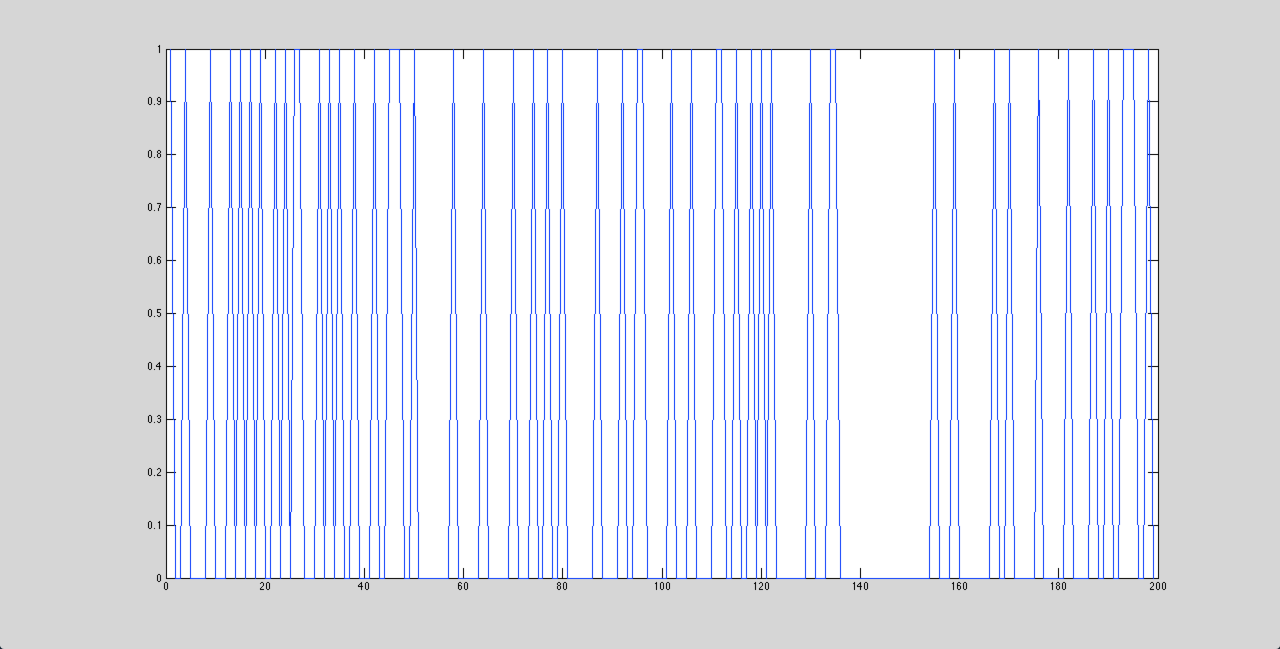
\includegraphics[width=0.3\textwidth]{images/exp/f=10.png}}
  \subfigure[F=20]{ \label{fig:subfig:b} %% label for second subfigure 
  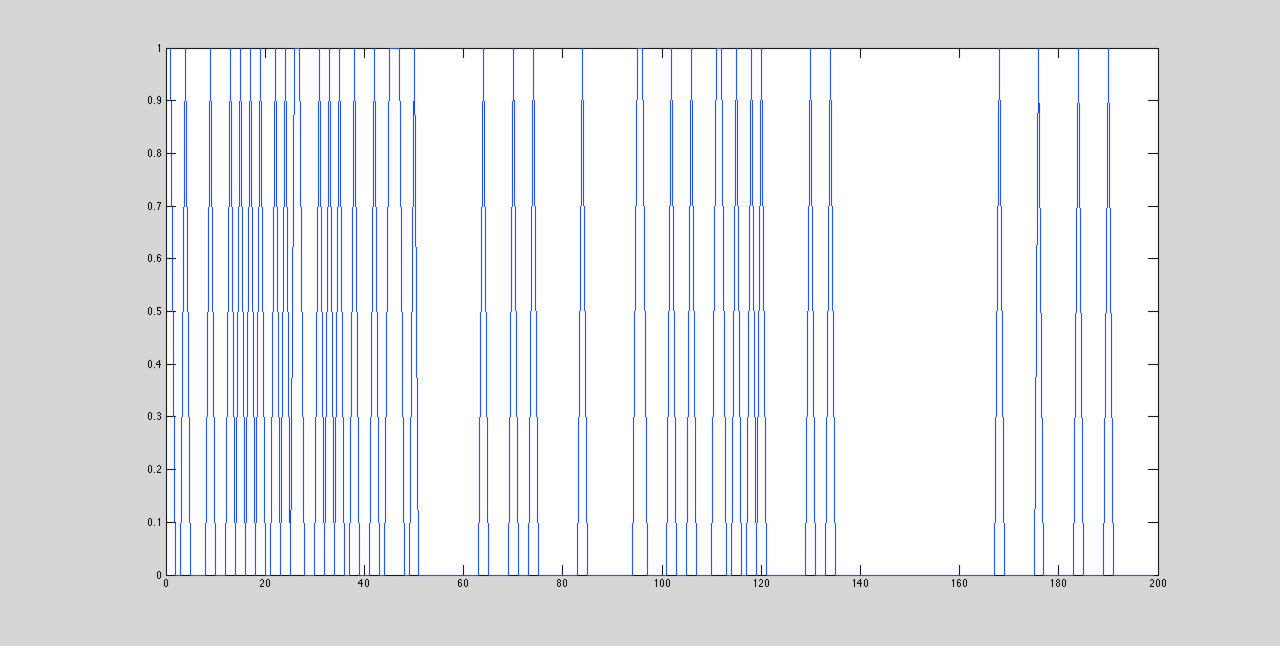
\includegraphics[width=0.3\textwidth]{images/exp/f=20.png}}  
  \subfigure[F=30]{ \label{fig:subfig:c} %% label for second subfigure 
  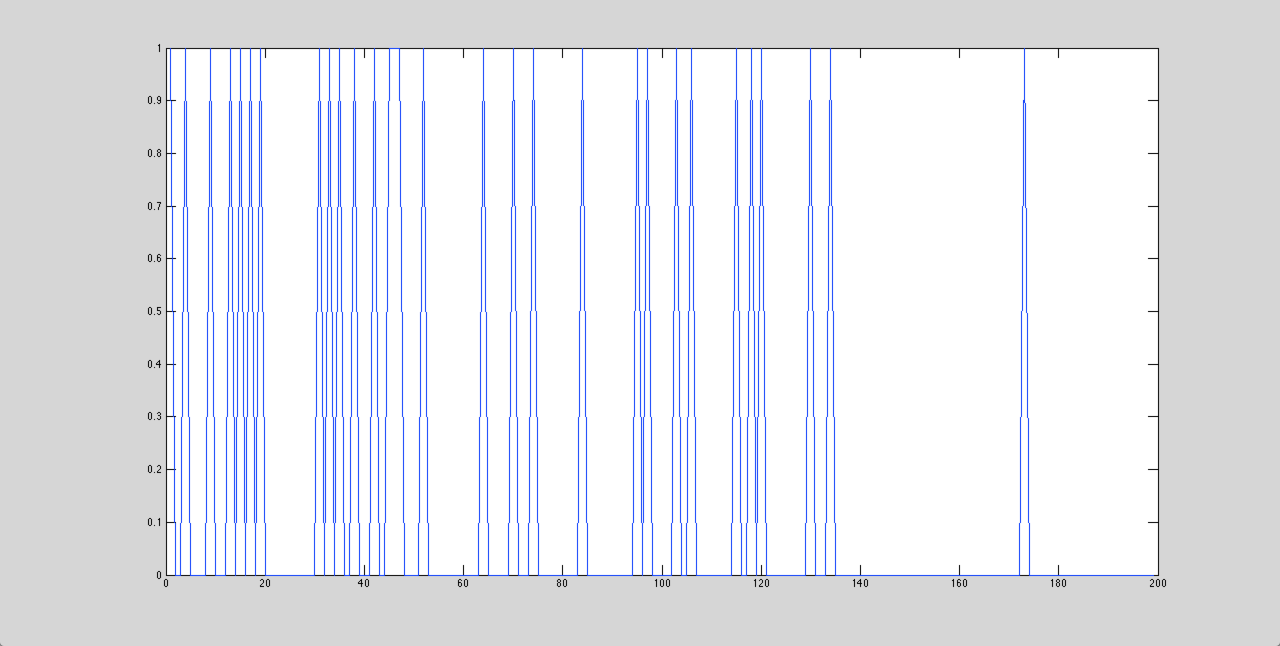
\includegraphics[width=0.3\textwidth]{images/exp/f=30.png}} 
  \caption{Different Factor}
   \label{fig:diff_f} %% label for entire figure 
\end{figure}

\subsubsection{Issues Encountered}
Basically, we can treat SA as a kind of EA. However, it has only one individual in the population. During the process of solving the optimization problem, SA encountered the same problem with SGA. As it doesn't have a large population, therefore, it can get stuck by local optimum. Another reason SA cannot get the global optimum easily is that it also treats the whole time interval as a whole. Therefore, when the traffic flow can be divided into several different traffic flows microscopically, it is not possible for SA to find the global optimum. 


\subsection{Mutable Time-interval Genetic Algorithm (MTGA)}
Our initial assumption was to work on time intervals during which the traffic flow is constant. However, after many simulations, we realized that even in a situation where the overall traffic flow is constant, the interaction between intersections and traffic lights creates a somewhat chaotic system where traffic flow at specific intersection can vary quite a bit. 

It became clear that we could achieve better results by further dividing our time intervals into smaller sub-intervals. We designed a new algorithm, in which the individuals also contain information about how to split the time interval: the Mutable Time-interval Genetic Algorithm (MTGA). It is a sort of Genetic Algorithm, and has the following features which will be explained later.
\begin{itemize}
	\item Hybrid Gene Type.
	\item No Crossover
	\item Special Mutation Type
\end{itemize}
The first and most important feature of MTGA is that it has a hybrid gene type. Below is how we encode the chromosome.
\begin{equation}
T_{1,1}, T_{1,2}, T_{1,3}, T_{1,4},T_{2,1}, T_{2,2}, T_{2,3}, T_{2,4},...,T_{n,1}, T_{n, 2},T_{n,3}, T_{n, 4},I_1, I_2, ..., I_n
\end{equation}
In the above equation, the a in the subscript of $T_{a,b}$ represents the time for the ath time interval and b represents the bth phase of a traffic light. For simplicity, in our example, we have only 1 traffic light. This traffic light has 4 phases which is the reason that b can be 4 at max. And we subdivide the whole time interval that we want to optimize our algorithm in into  sub regions. $I_1, I_2, ...$ represents the length of each phase respectively. One thing that we have to mention is that the sum of $I_2, I_2, ...$ should be a fixed constant which represents the length of the time interval we want to estimate our algorithm in. It can be expressed like this:
\begin{equation}
\label{equ_sum_fixed}
I_2 + I_2 + I_3 + ... + I_n = T
\end{equation} 
where T represents the time interval between start time and end time.\\

Another important feature is that you cannot really perform crossover in MTGA although they align with each other very well. The reason comes from its special chromosome. Because we usually want to optimize the traffic light for a fixed time interval, therefore, $I_1 + I_2 + ... + I_n$ has to be fixed to the length of the time interval. If we perform crossover between two individuals, the sum of these numbers will change. Although we can find a way to perform crossover between two individuals, we didn't add this feature into our algorithm.

The last feature is that we have to perform special mutation in MTGA. In the first part of the chromosome, we can perform mutation as usual. However as stated above, we have to change at least two genes at together because of equation \ref{equ_sum_fixed}. For example, we want to change ${I_1}$. Let's assume that, previously, we have $I_1 = 40, I_2 = 40, I_3 = 100$. If we try to mutate$I_1$ from 40 to 20. We can set $I_1 = 20$. However, we have to do either $I_2=60$ or $I_3=120$ as well in order to keep consistent to equation \ref{equ_sum_fixed}. 


\subsection{Fixed Time-interval Genetic Algorithm (FTGA)}
Based on the above algorithm, we came up with a modified version of the MTGA: the Fixed Time-interval Genetic Algorithm (FTGA). The simple idea is to get rid of $I_1, I_2, ..., I_n$ which are encoded in equation\ref{equ_sum_fixed}. We will ourselves decide to split the time interval into a number of equal-length sub-intervals: $I_1=I_2=...=I_n$. This means that we don't need to store the intervals in the chromosomes anymore. The chromosome's representation is the following:
\begin{equation}
T_{1,1}, T_{1,2}, T_{1,3}, T_{1,4},T_{2,1}, T_{2,2}, T_{2,3}, T_{2,4},...,T_{n,1}, T_{n, 2},T_{n,3}, T_{n, 4}
\end{equation}
By limiting $T_{a,b}$ to a certain domain such as (1,100), we don't even have to perform the special mutation either. What we can do with normal Genetic Algorithm can be applied to this chromosome as well. And another important feature that FTGA has is that it has fewer parameters which means it takes us a shorter time to get the result. 


\section{Experiment \& Result}
\subsection{Result}
During these experiments, we fixed the population size of SGA, FTGA and MTGA to 20 and the number of offspring size to 6 which means that during each generation, we have to evaluate 26 individuals. We fixed the number of generations to 40. And we chose 40 random number sequences to evaluate these algorithms. Therefore, with 1 random number sequence, we have to evaluate $40 * 26 = 1040$ individuals. And we run each algorithm 40 times.

In order to measure the performance of all these algorithms, we fixed the traffic flow, number of simulation step, and the total number of cars input into the simulator. Therefore, we know exactly the global optimum of this problem and we try to find out whether each algorithm can achieve it.


\subsubsection{Successful Rate}
Figure \ref{fig:success_rate} shows the successful rate of each algorithm. We define the success of an algorithm as equation \ref{equ:success}
\begin{equation}
\begin{split}
&\text{\emph{IF} best fitness = global optimum} \\
&\text{\hspace{2em}\emph{RETURN} \emph{True}}\\
&\emph{ELSE}\\
&\text{\hspace{2em}\emph{RETURN} \emph{False}}\\
\label{equ:success}
\end{split}
\end{equation}
According to the experiment setup stated before, we counted the number of successes for each algorithm and plotted them in Figure \ref{fig:success_rate}

\begin{figure}[htbp]
\centering
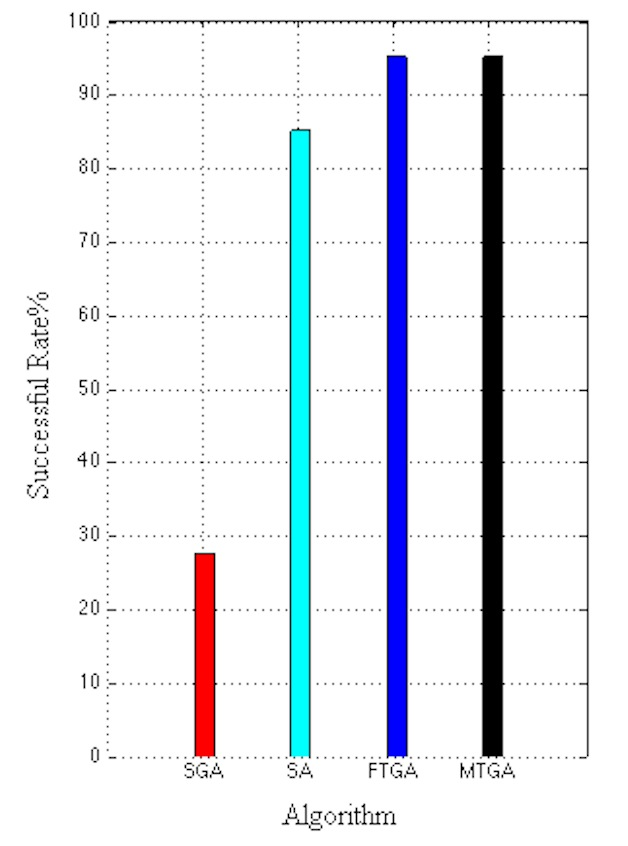
\includegraphics[width=0.5\textwidth]{images/exp/successful_rate.png}
\label{fig:success_rate}
\caption{Successful Rate}
\end{figure}

\subsubsection{Average Fitness}
During these experiments, we also recorded the average fitness of each algorithm. We analyzed all the data we recorded. Figure \ref{fig:avg_fitness} shows a representative run of each algorithm. From this figure, we can see that the average fitness of FTGA is the best among the four algorithms for most of the time. SGA starts at a low fitness and increases quickly. The average fitness of SA tends to fluctuate. In this case, MTGA remains a relatively high average fitness. We can see that, although MTGA is more flexible than FTGA, it tends to have a lower average. The reason we conclude is that since MTGA has a more flexible chromosome, crossover and mutation are more likely to destruct its good individuals. And the chromosome of FTGA has fewer genes, therefore it is less likely to be affected by these effects.

\begin{figure}[htbp]
\centering
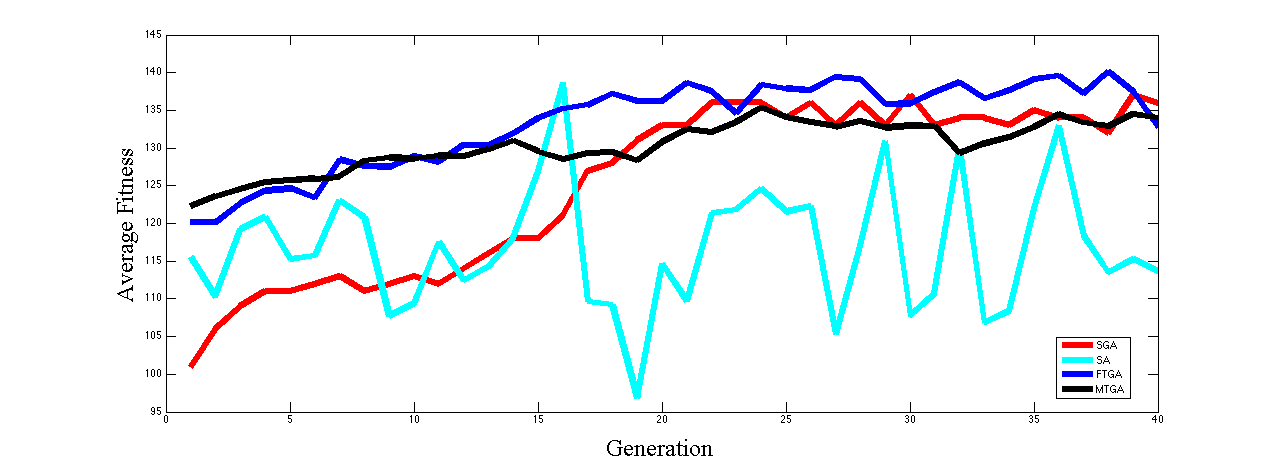
\includegraphics[width=\textwidth]{images/exp/avg_fitness.png}
\label{fig:avg_fitness}
\caption{Average Fitness}
\end{figure}

\subsubsection{Best Fitness}
Besides average fitness, we measured the best fitness during the process. Figure \ref{fig:best_fitness} shows the result of this experiment. We can find out that even the average fitness of MTGA may be lower than FTGA, it is more likely to get the global optimum since it is a more precise representation of the problem. SGA tends to behave badly in the beginning. As time goes by, the best fitness it can achieve increases dramatically. SA can achieve its best fitness at any time during its process and it is hard to predict. 

\begin{figure}[h]
\centering
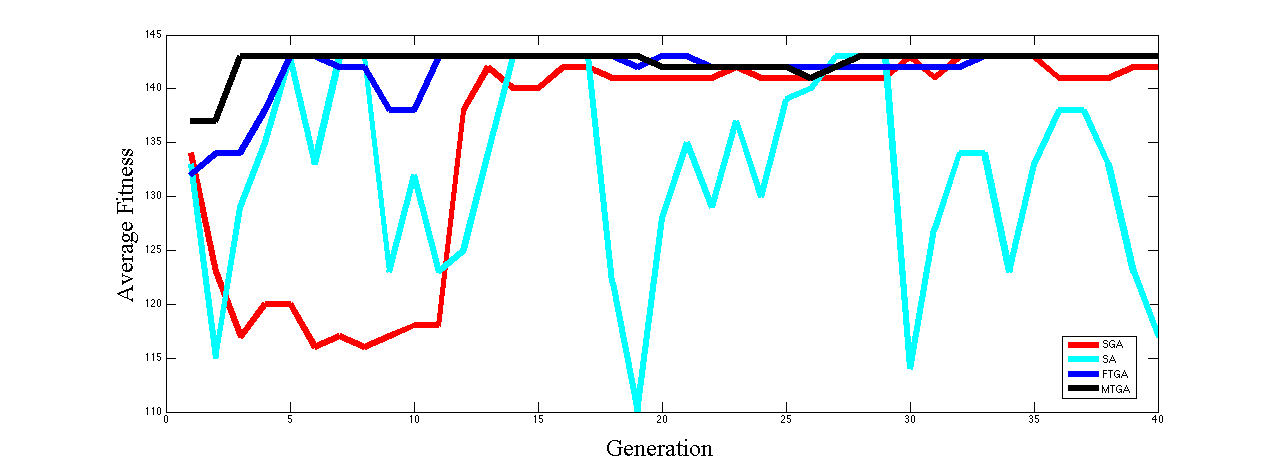
\includegraphics[width=\textwidth]{images/exp/best_all.png}
\label{fig:best_fitness}
\caption{Best Fitness}
\end{figure}

\subsection{Conclusion}
Having investigated a lot work done by others, we found out that almost all of them are based on traditional methods which treat the time interval as a whole. It is a trivial way to solve the problem since EA can deal with this situation perfectly with the unnecessary constraint that the time interval cannot be subdivided. Actually, when it comes to real-world, unpredictable accident happens. Therefore, these factors can affect the traffic flow from time to time. We human beings may not find the subtle difference easily. However, properly designed algorithms are able to find them out.

SGA and SA represent two kinds of traditional algorithms that treat the time interval we want to optimize as a whole. They showed some ability to improve the traffic flow. However, they reach their bottlenecks easily. In some scenarios, they can never get the global optimum. 

FTGA and MTGA are specially designed for subdividing the whole time interval into sub-regions. Therefore, they both have the ability to improve the max fitness that SGA and SA and achieve. Although they use different approaches to divide the time interval, they turned out to be feasible to find the global optimum. 

\begin{table}
\centering
\renewcommand\arraystretch{2}
    \begin{tabular}{|l|l|l|}
    \hline
    \textbf{Algorithm} & \textbf{Maximum Fitness} & \textbf{Success Times} \\ \hline
    Original  & 123             & N/N             \\ \hline
    SGA       & 143             & 11/40           \\ \hline
    SA        & 143             & 34/40           \\ \hline
    FTGA      & 143             & 38/40           \\ \hline
    MTGA      & 143             & 38/40           \\ \hline
    \end{tabular}
    \caption {Performance of Algorithms}
    \label{tab:pa}
\end{table}

According to the result from table \ref{tab:pa}, we can see that, SGA and SA can optimize the traffic to a certain extent. Although SGA and SA and achieve the global optimum at times, they are not guaranteed to find ti. As FTGA and MTGA have the ability to subdivide the whole time interval into smaller ones, they can further improve the traffic timing. Therefore, they are more likely to find the global optimum. Also, we have stated that FTGA is a simplified version of MTGA. However, it behaves almost as well as MTGA. And it is much easier to implement.


\subsubsection*{Acknowledgments}

We take this opportunity to express our profound gratitude and deep regards to our teacher Professor Jason D Lohn, Associate Research Professor in the Dept. of Electrical and Computer Engineering in Carnegie Mellon University, for his exemplary guidance, monitoring and constant encouragement throughout this report. In developing the ideas used in optimizing traffic lights timing with evolutionary algorithm, we have received helpful inspiration from him. The blessing, help and guidance given by him time to time shall carry us a long way in the journey of our graduate study.

We also thank Irina Brinster, full-time PhD in Carnegie Mellon University, for her technical support and valuable information, which helped us in completing this project  through various stages.

Thanks also go out the the developers of the SUMO simulator.

\subsubsection*{References}

\small{
[1] Walters, Ken (2012) Smart Traffic Signals Pilot Results: Pollution Plunges, Traffic Clogs Cleared. \url{http://www.cmu.edu/news/stories/archives/2012/september/sept24_smarttrafficsignals.html}

[2] Xiaoming You (2008) Urban intelligent traffic operation optimization control strategy based on real-corded evolutionary algorithm. \url{http://ieeexplore.ieee.org/xpl/login.jsp?tp=&arnumber=4598052}

[3] Jansson, Gustaf (2010) Traffic Control with Standard Genetic Algorithm \url{http://publications.lib.chalmers.se/records/fulltext/138247.pdf}

[4] Sanchez Medina, Javier J (2008) Evolutionary Computation Applied to Urban Traffic Optimization \url{http://cdn.intechopen.com/pdfs/5247/InTech-Evolutionary_computation_applied_to_urban_traffic_optimization.pdf}
}
\end{document}
